\documentclass{report}
\usepackage{graphicx, tikz-cd} % Required for inserting images
\usepackage{amsmath, amssymb, amsthm, amsfonts, siunitx, physics}
\AtBeginDocument{\RenewCommandCopy\qty\SI}
\usepackage[version=4]{mhchem}
\usepackage[most,many,breakable]{tcolorbox}
\usepackage{xcolor, fancyhdr, varwidth}
\usepackage[Glenn]{fncychap}
%Options: Sonny, Lenny, Glenn, Conny, Rejne, Bjarne, Bjornstrup
\usepackage{hyperref, cleveref}
\usepackage{icomma, enumitem} %comma as decimal and continue enumerate with [resume]
%%%%%%%%%%%%%%%%%%%%%%%%%%%%%%
% SELF MADE COLORS
%%%%%%%%%%%%%%%%%%%%%%%%%%%%%%
\definecolor{myg}{RGB}{56, 140, 70}
\definecolor{myb}{RGB}{45, 111, 177}
\definecolor{myr}{RGB}{199, 68, 64}
\definecolor{mytheorembg}{HTML}{F2F2F9}
\definecolor{mytheoremfr}{HTML}{00007B}
\definecolor{mylenmabg}{HTML}{FFFAF8}
\definecolor{mylenmafr}{HTML}{983b0f}
\definecolor{mypropbg}{HTML}{f2fbfc}
\definecolor{mypropfr}{HTML}{191971}
\definecolor{myexamplebg}{HTML}{F2FBF8}
\definecolor{myexamplefr}{HTML}{88D6D1}
\definecolor{myexampleti}{HTML}{2A7F7F}
\definecolor{mydefinitbg}{HTML}{E5E5FF}
\definecolor{mydefinitfr}{HTML}{3F3FA3}
\definecolor{notesgreen}{RGB}{0,162,0}
\definecolor{myp}{RGB}{197, 92, 212}
\definecolor{mygr}{HTML}{2C3338}
\definecolor{myred}{RGB}{127,0,0}
\definecolor{myyellow}{RGB}{169,121,69}
\definecolor{myexercisebg}{HTML}{F2FBF8}
\definecolor{myexercisefg}{HTML}{88D6D1}
%%%%%%%%%%%%%%%%%%%%%%%%%%%%%%%%%%%%%%%%%%%%%%%%%%%%%%%%%%%%%%%%%%%%%%
% Box environments for theorems and problems
%%%%%%%%%%%%%%%%%%%%%%%%%%%%%%%%%%%%%%%%%%%%%%%%%%%%%%%%%%%%%%%%%%%%%
\setlength{\parindent}{1cm}
%================================
% Question BOX
%================================
\makeatletter
\newtcbtheorem{question}{Opgave}{enhanced,
	breakable,
	colback=white,
	colframe=myb!80!black,
	attach boxed title to top left={yshift*=-\tcboxedtitleheight},
	fonttitle=\bfseries,
	title={#2},
	boxed title size=title,
	boxed title style={%
			sharp corners,
			rounded corners=northwest,
			colback=tcbcolframe,
			boxrule=0pt,
		},
	underlay boxed title={%
			\path[fill=tcbcolframe] (title.south west)--(title.south east)
			to[out=0, in=180] ([xshift=5mm]title.east)--
			(title.center-|frame.east)
			[rounded corners=\kvtcb@arc] |-
			(frame.north) -| cycle;
		},
	#1
}{def}
\makeatother
%================================
% DEFINITION BOX
%================================

\newtcbtheorem[]{Definition}{Definition}{enhanced,
	before skip=2mm,after skip=2mm, colback=red!5,colframe=red!80!black,boxrule=0.5mm,
	attach boxed title to top left={xshift=1cm,yshift*=1mm-\tcboxedtitleheight}, varwidth boxed title*=-3cm,
	boxed title style={frame code={
					\path[fill=tcbcolback]
					([yshift=-1mm,xshift=-1mm]frame.north west)
					arc[start angle=0,end angle=180,radius=1mm]
					([yshift=-1mm,xshift=1mm]frame.north east)
					arc[start angle=180,end angle=0,radius=1mm];
					\path[left color=tcbcolback!60!black,right color=tcbcolback!60!black,
						middle color=tcbcolback!80!black]
					([xshift=-2mm]frame.north west) -- ([xshift=2mm]frame.north east)
					[rounded corners=1mm]-- ([xshift=1mm,yshift=-1mm]frame.north east)
					-- (frame.south east) -- (frame.south west)
					-- ([xshift=-1mm,yshift=-1mm]frame.north west)
					[sharp corners]-- cycle;
				},interior engine=empty,
		},
	fonttitle=\bfseries,
	title={#2},#1}{def}
\newtcbtheorem[]{definition}{Definition}{enhanced,
	before skip=2mm,after skip=2mm, colback=red!5,colframe=red!80!black,boxrule=0.5mm,
	attach boxed title to top left={xshift=1cm,yshift*=1mm-\tcboxedtitleheight}, varwidth boxed title*=-3cm,
	boxed title style={frame code={
					\path[fill=tcbcolback]
					([yshift=-1mm,xshift=-1mm]frame.north west)
					arc[start angle=0,end angle=180,radius=1mm]
					([yshift=-1mm,xshift=1mm]frame.north east)
					arc[start angle=180,end angle=0,radius=1mm];
					\path[left color=tcbcolback!60!black,right color=tcbcolback!60!black,
						middle color=tcbcolback!80!black]
					([xshift=-2mm]frame.north west) -- ([xshift=2mm]frame.north east)
					[rounded corners=1mm]-- ([xshift=1mm,yshift=-1mm]frame.north east)
					-- (frame.south east) -- (frame.south west)
					-- ([xshift=-1mm,yshift=-1mm]frame.north west)
					[sharp corners]-- cycle;
				},interior engine=empty,
		},
	fonttitle=\bfseries,
	title={#2},#1}{def}

\newtcbtheorem{theo}%
    {Theorem}{}{theorem}
\newtcolorbox{prob}[1]{colback=red!5!white,colframe=red!50!black,fonttitle=\bfseries,title={#1}}
%================================
% NOTE BOX
%================================

\usetikzlibrary{arrows,calc,shadows.blur}
\tcbuselibrary{skins}
\newtcolorbox{note}[1][]{%
	enhanced jigsaw,
	colback=gray!20!white,%
	colframe=gray!80!black,
	size=small,
	boxrule=1pt,
	title=\textbf{Note:},
	halign title=flush center,
	coltitle=black,
	breakable,
	drop shadow=black!50!white,
	attach boxed title to top left={xshift=1cm,yshift=-\tcboxedtitleheight/2,yshifttext=-\tcboxedtitleheight/2},
	minipage boxed title=1.5cm,
	boxed title style={%
			colback=white,
			size=fbox,
			boxrule=1pt,
			boxsep=2pt,
			underlay={%
					\coordinate (dotA) at ($(interior.west) + (-0.5pt,0)$);
					\coordinate (dotB) at ($(interior.east) + (0.5pt,0)$);
					\begin{scope}
						\clip (interior.north west) rectangle ([xshift=3ex]interior.east);
						\filldraw [white, blur shadow={shadow opacity=60, shadow yshift=-.75ex}, rounded corners=2pt] (interior.north west) rectangle (interior.south east);
					\end{scope}
					\begin{scope}[gray!80!black]
						\fill (dotA) circle (2pt);
						\fill (dotB) circle (2pt);
					\end{scope}
				},
		},
	#1,
}

%%%%%%%%%%%%%%%%%%%%%%%%%%%%%%%%%%%%%%%%%%%%%%%%%%%%%%%%%%%%%%%%%
% SELF MADE COMMANDS
%%%%%%%%%%%%%%%%%%%%%%%%%%%%%%
\newcommand{\sol}{\setlength{\parindent}{0cm}\textbf{\textit{Løsning:}}\setlength{\parindent}{1cm}}
%%%%%%%%%%%%%%%%%%%%%%%%%%%%%%%%%
\usepackage[tmargin=2cm,rmargin=1in,lmargin=1in,margin=0.85in,bmargin=2cm,footskip=.2in]{geometry}\pagestyle{fancy}
\lhead{Minrui Kevin Zhou 2.b}
\rhead{H4: Mekanik}

\title{H4: Mekanik\\
{\Large \textbf{2.b Fysik A}}}
\author{Kevin Zhou}
\date{September 2023}

\begin{document}
\maketitle
\chapter{Den elektriske racerbil TC-X}
\begin{question}{}{}
  Elbilen TC-X er en danskbygget racerbil. Bilen er bygget til at accelerere lynhurtigt på en kort strækning.
I august 2017 slog den rekorden som verdens hurtigste eldrevne bil. Under rekordforsøget tilbagelagde elbilen TC-X afstanden $201,17 \; \unit{m}$ på $4,897 \; \unit{s}$.
  \begin{itemize}
    \item[a.] Bestem elbilens gennemsnitlige fart under rekordforsøget.
  \end{itemize}
\end{question}
\sol \\
Den gennemsnitlige fart for elbilen er blot strækningen over tiden.
\[
fart_{bil} = \frac{s}{t} = \frac{201,17 \; \unit{m}}{4,897 \; \unit{s}} \approx 41,08 \; \unit{m/s}
\] 
Altså er bilens gennemsnitlige fart $41,08 \; \unit{m/s}$

\begin{question}{}{}
Under rekordforsøget accelererede elbilen TC-X fra hvile til farten $100 \; \unit{km/h}$ med en gennemsnitlig acceleration med størrelsen $25,3 \; \unit{m/s^2}$ 
\begin{itemize}
  \item[b.] Hvor lang tid ville det tage elbilen TC-X at opnå farten $100 \; \unit{km/h}$, hvis dens acceleration havde haft den nævnte værdi siden start? ("0-100 på ? sekunder") 
\end{itemize}
\end{question}
\sol \\ 
Accelerationen i dette tilfælde er ment som ændringen af farten. Vi kan da regne tiden ud.
\begin{equation*}
\begin{split}
t = \frac{fart}{a} &= \frac{100 \; \unit{km/h}}{25,3 \; \unit{m/s^2}}\\ 
  &= \frac{\frac{100}{3,6}\;\unit{m/s}}{{25,3 \; \unit{m/s^2}}}\\ 
  &\approx 1,10 \;\unit{s}
\end{split} 
\end{equation*}
Altså tager det TC-X $1,10 \;\unit{s}$ at opnå farten $100 \; \unit{km/h}$. 

\pagebreak
\begin{question}{}{}
Kort efter starten af rekordforsøget målte man bilens fart. Tabellen viser bilens fart $v$ som funktion af tiden $t$ efter start.
$$
\begin{array}{|l|c|c|c|c|c|c|c|}
  \hline \text { tid/s } & 0,700 & 0,800 & 0,900 & 1,00 & 1,10 & 1,20 & 1,30 \\
  \hline \text { fart/(\unit{m/s}) } & 20,2 & 22,3 & 24,3 & 26,1 & 27,8 & 29,4 & 30,9 \\
\hline
\end{array}
$$
\begin{itemize}
  \item[c.] Bestem ved hjælp af tabellens data (uden at tegne en graf) størrelsen af bilens acceleration $0,800 \;\unit{s}$ efter start.
\end{itemize}
\end{question}
\sol \\ 
Vi benytter numerisk differentiation til at estimere bilens acceleration $\left(\dv{t}(fart)\right)$ $0,800 \;\unit{s}$ efter start.
\[
a \approx \frac{24,3\;\unit{m/s}-20,2\;\unit{m/s}}{0,900\;\unit{s}-0,700\;\unit{s}} = 20,5\;\unit{m/s^2}
\] 
Altså er bilens acceleration cirka $20,5\;\unit{m/s^2}$ efter $0,800 \;\unit{s}$.

\begin{question}{}{}
\begin{itemize}
  \item[d.] Indsæt tabellens data i en Logger Pro-fil, og tegn en (t, v)-graf.
  \item[e.] Lav et lineært fit i Logger Pro, og opskriv forskriften for fartfunktionen $v(t)$ ud fra denne model. Hvor godt passer modellen med data?
  \item[f.] Lav så et fit med et andengradspolynomium, og opskriv forskriften for fartfunktionen $v(t)$ ud fra denne model. Hvor godt passer modellen med data?
\end{itemize}
\end{question}
\sol \\ 
I \cref{fig:1} ses tabellens data indsat i Logger Pro, hvorefter et lineært fit er lavet. Denne passer meget godt. Ifølge denne model er fartfunktionen
\[
v(t)=17,8\;\unit{m/s^2}\cdot t + 8,07\;\unit{m/s}
\] 
\begin{figure}[h]
\begin{center}
  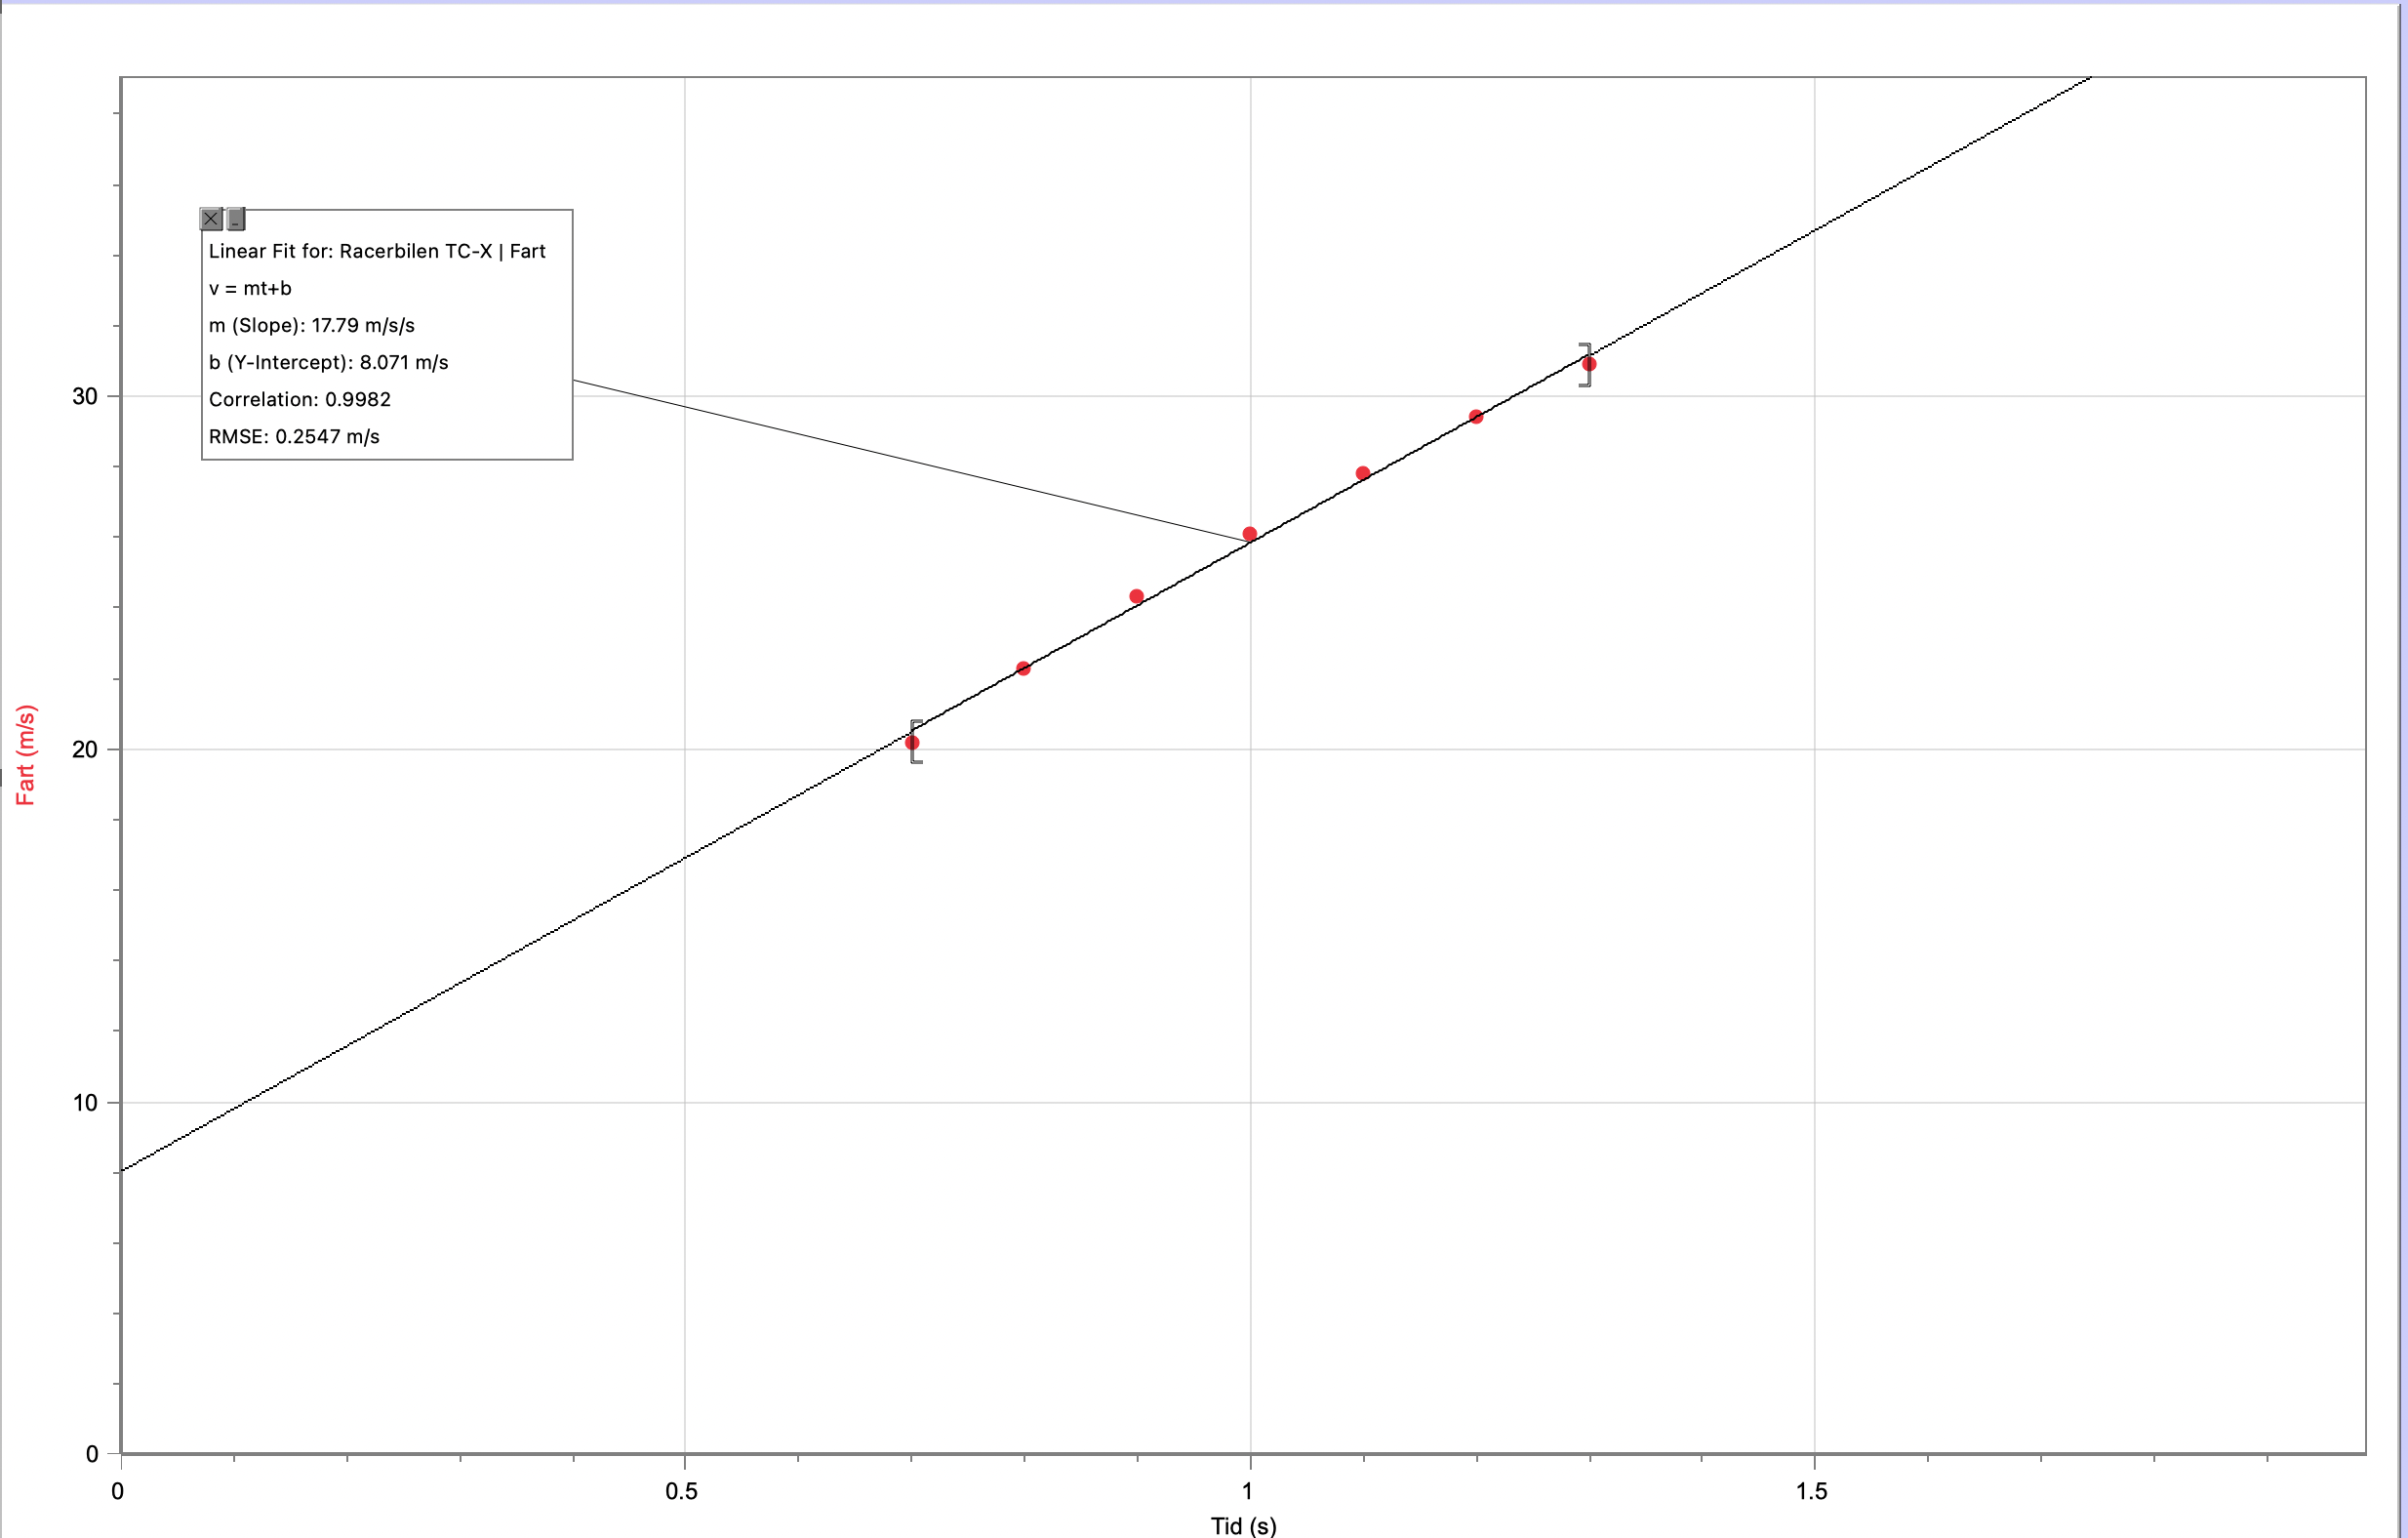
\includegraphics[scale=0.3]{H4_1.png}
\end{center}
\caption{Lineært fit i Logger Pro}
\label{fig:1}
\end{figure}
\linebreak
I \cref{fig:2} ses et kvadratisk fit lavet i Logger Pro. Denne model passer perfekt med data. Ifølge denne model er fartfunktionen
\[
v(t)=-6,19\;\unit{m/s^3}\cdot t^3 + 30,1\;\unit{m/s^2} \cdot t^2 + 2,12\;\unit{m/s}
\] 
\begin{figure}[h]
\begin{center}
  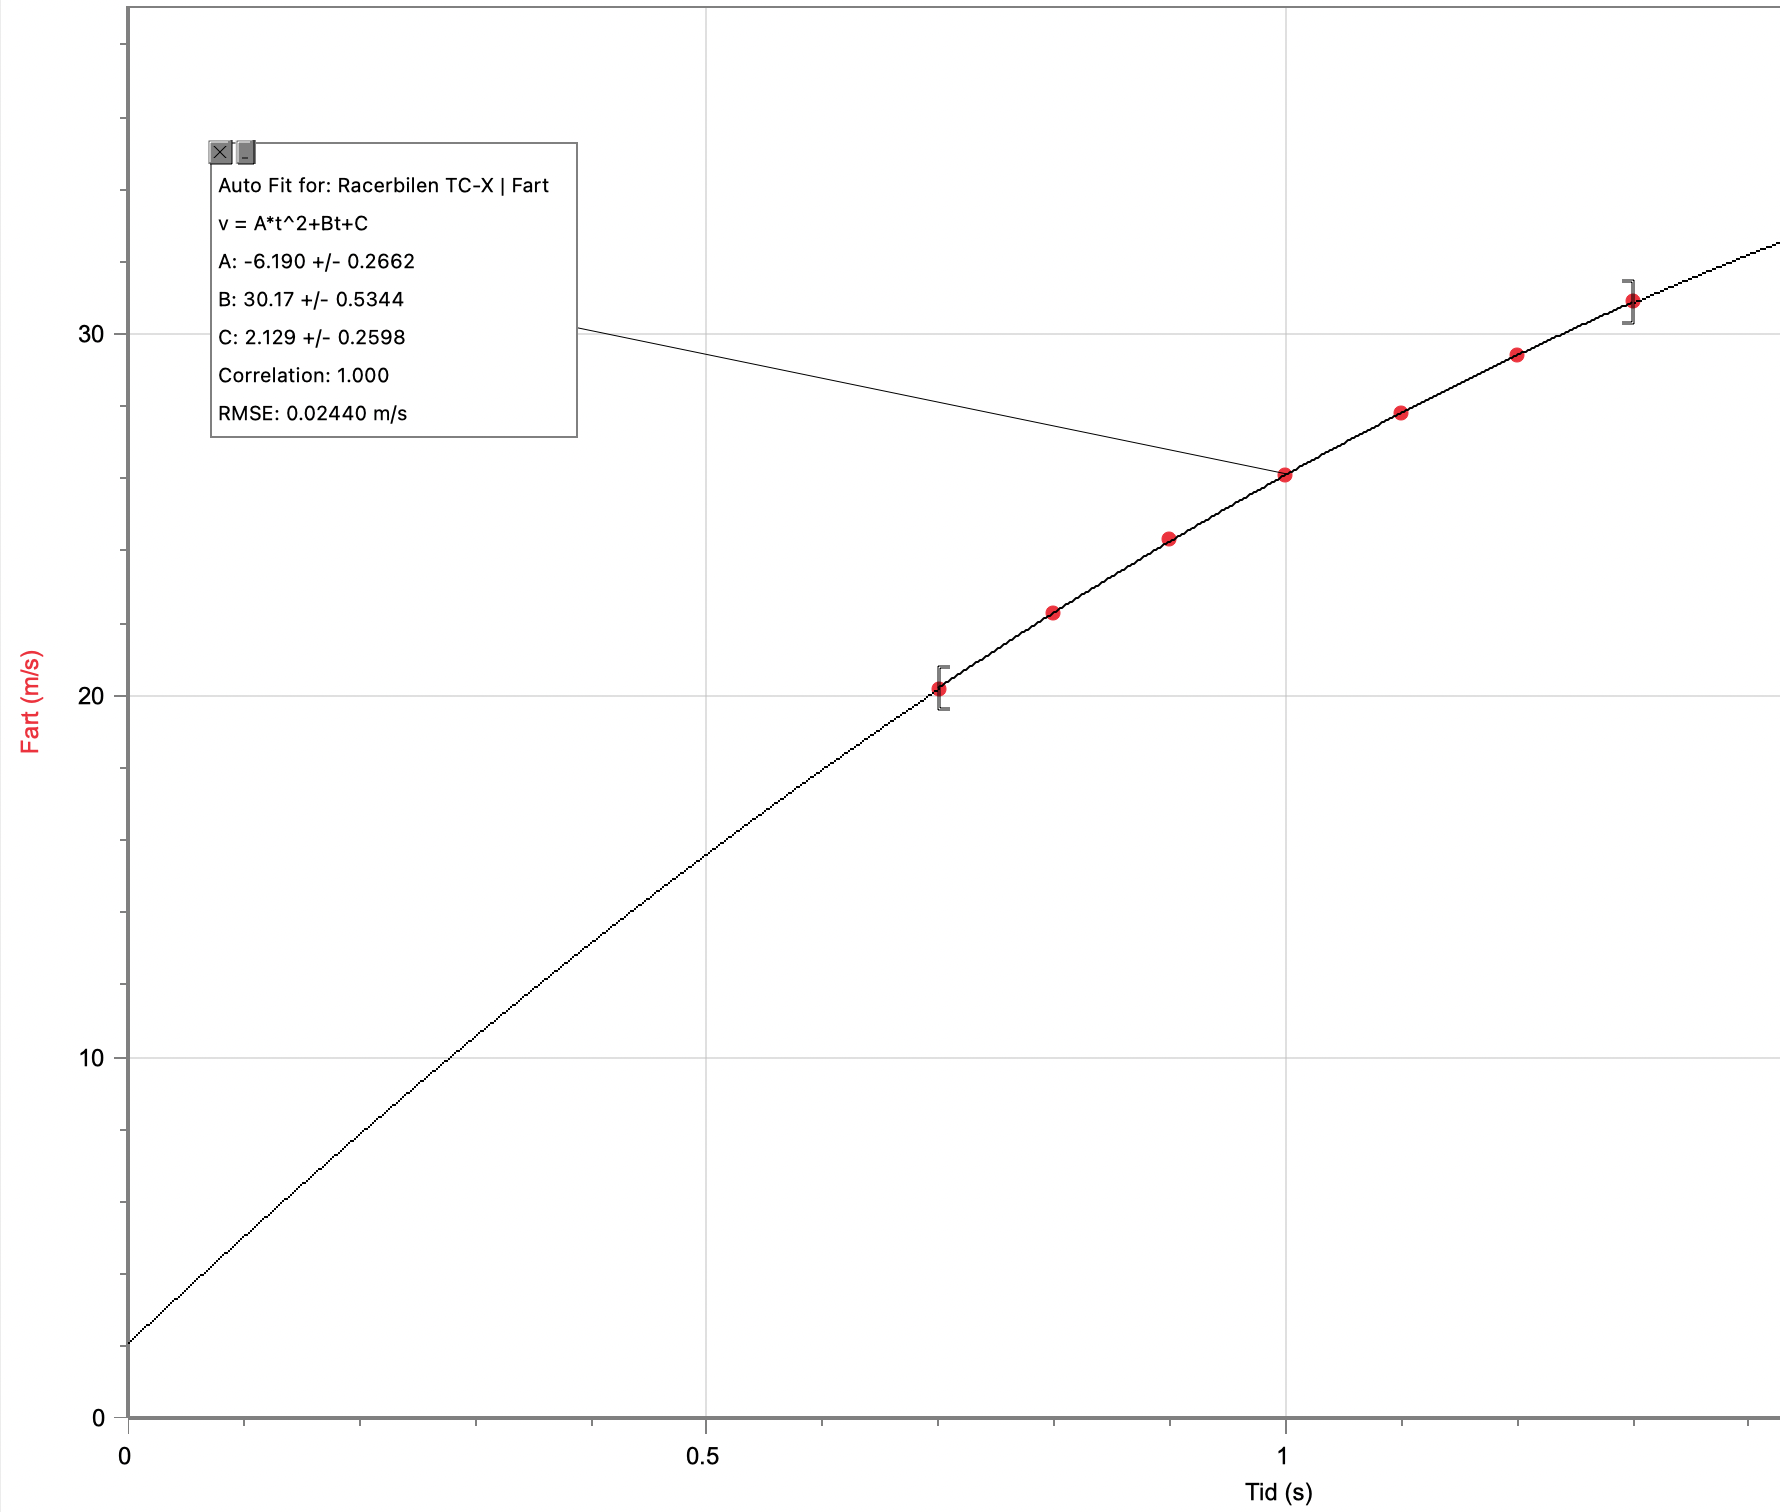
\includegraphics[scale=0.3]{H4_2.png}
\end{center}
\caption{Kvadratisk fit i Logger Pro}
\label{fig:2}
\end{figure}

\begin{question}{}{}
\begin{itemize}
  \item[g.] Ovenfor står der "Under rekordforsøget accelererede elbilen TC-X fra hvile ..." - så hvilken værdi har $v(0\;\unit{s})$? Hvordan passer det med de to modeller ovenfor?
  \item[h.] Tilføj nu et passende punkt mere til tabellen i Logger Pro, så den passer med citatet. Forklar, hvorfor det giver bedre fysisk mening end de to foregående.
\end{itemize}
\end{question}
\sol \\ 
Siden bilen accelererede fra hvile, så må følgende, per definition af hvile, gælde.
\[
v(0\;\unit{s})=0\;\unit{m/s}
\] 
Dette passer umiddelbart ikke med de to ovenstående modeller, da farten ved $\qty{0}{s}$ ikke er $\qty{0}{m/s}$ ifølge modellerne.\par
I \cref{fig:3} ses fittet med andengradspolynomiet efter tilføjelse af punktet $(0,0)$. Dette ville give bedre fysisk mening, da bilen så har farten $\qty{0}{m/s}$ ved start, hvilket netop er det, der menes ved, at bilen accelererede fra hvile.
\begin{figure}[h]
\begin{center}
  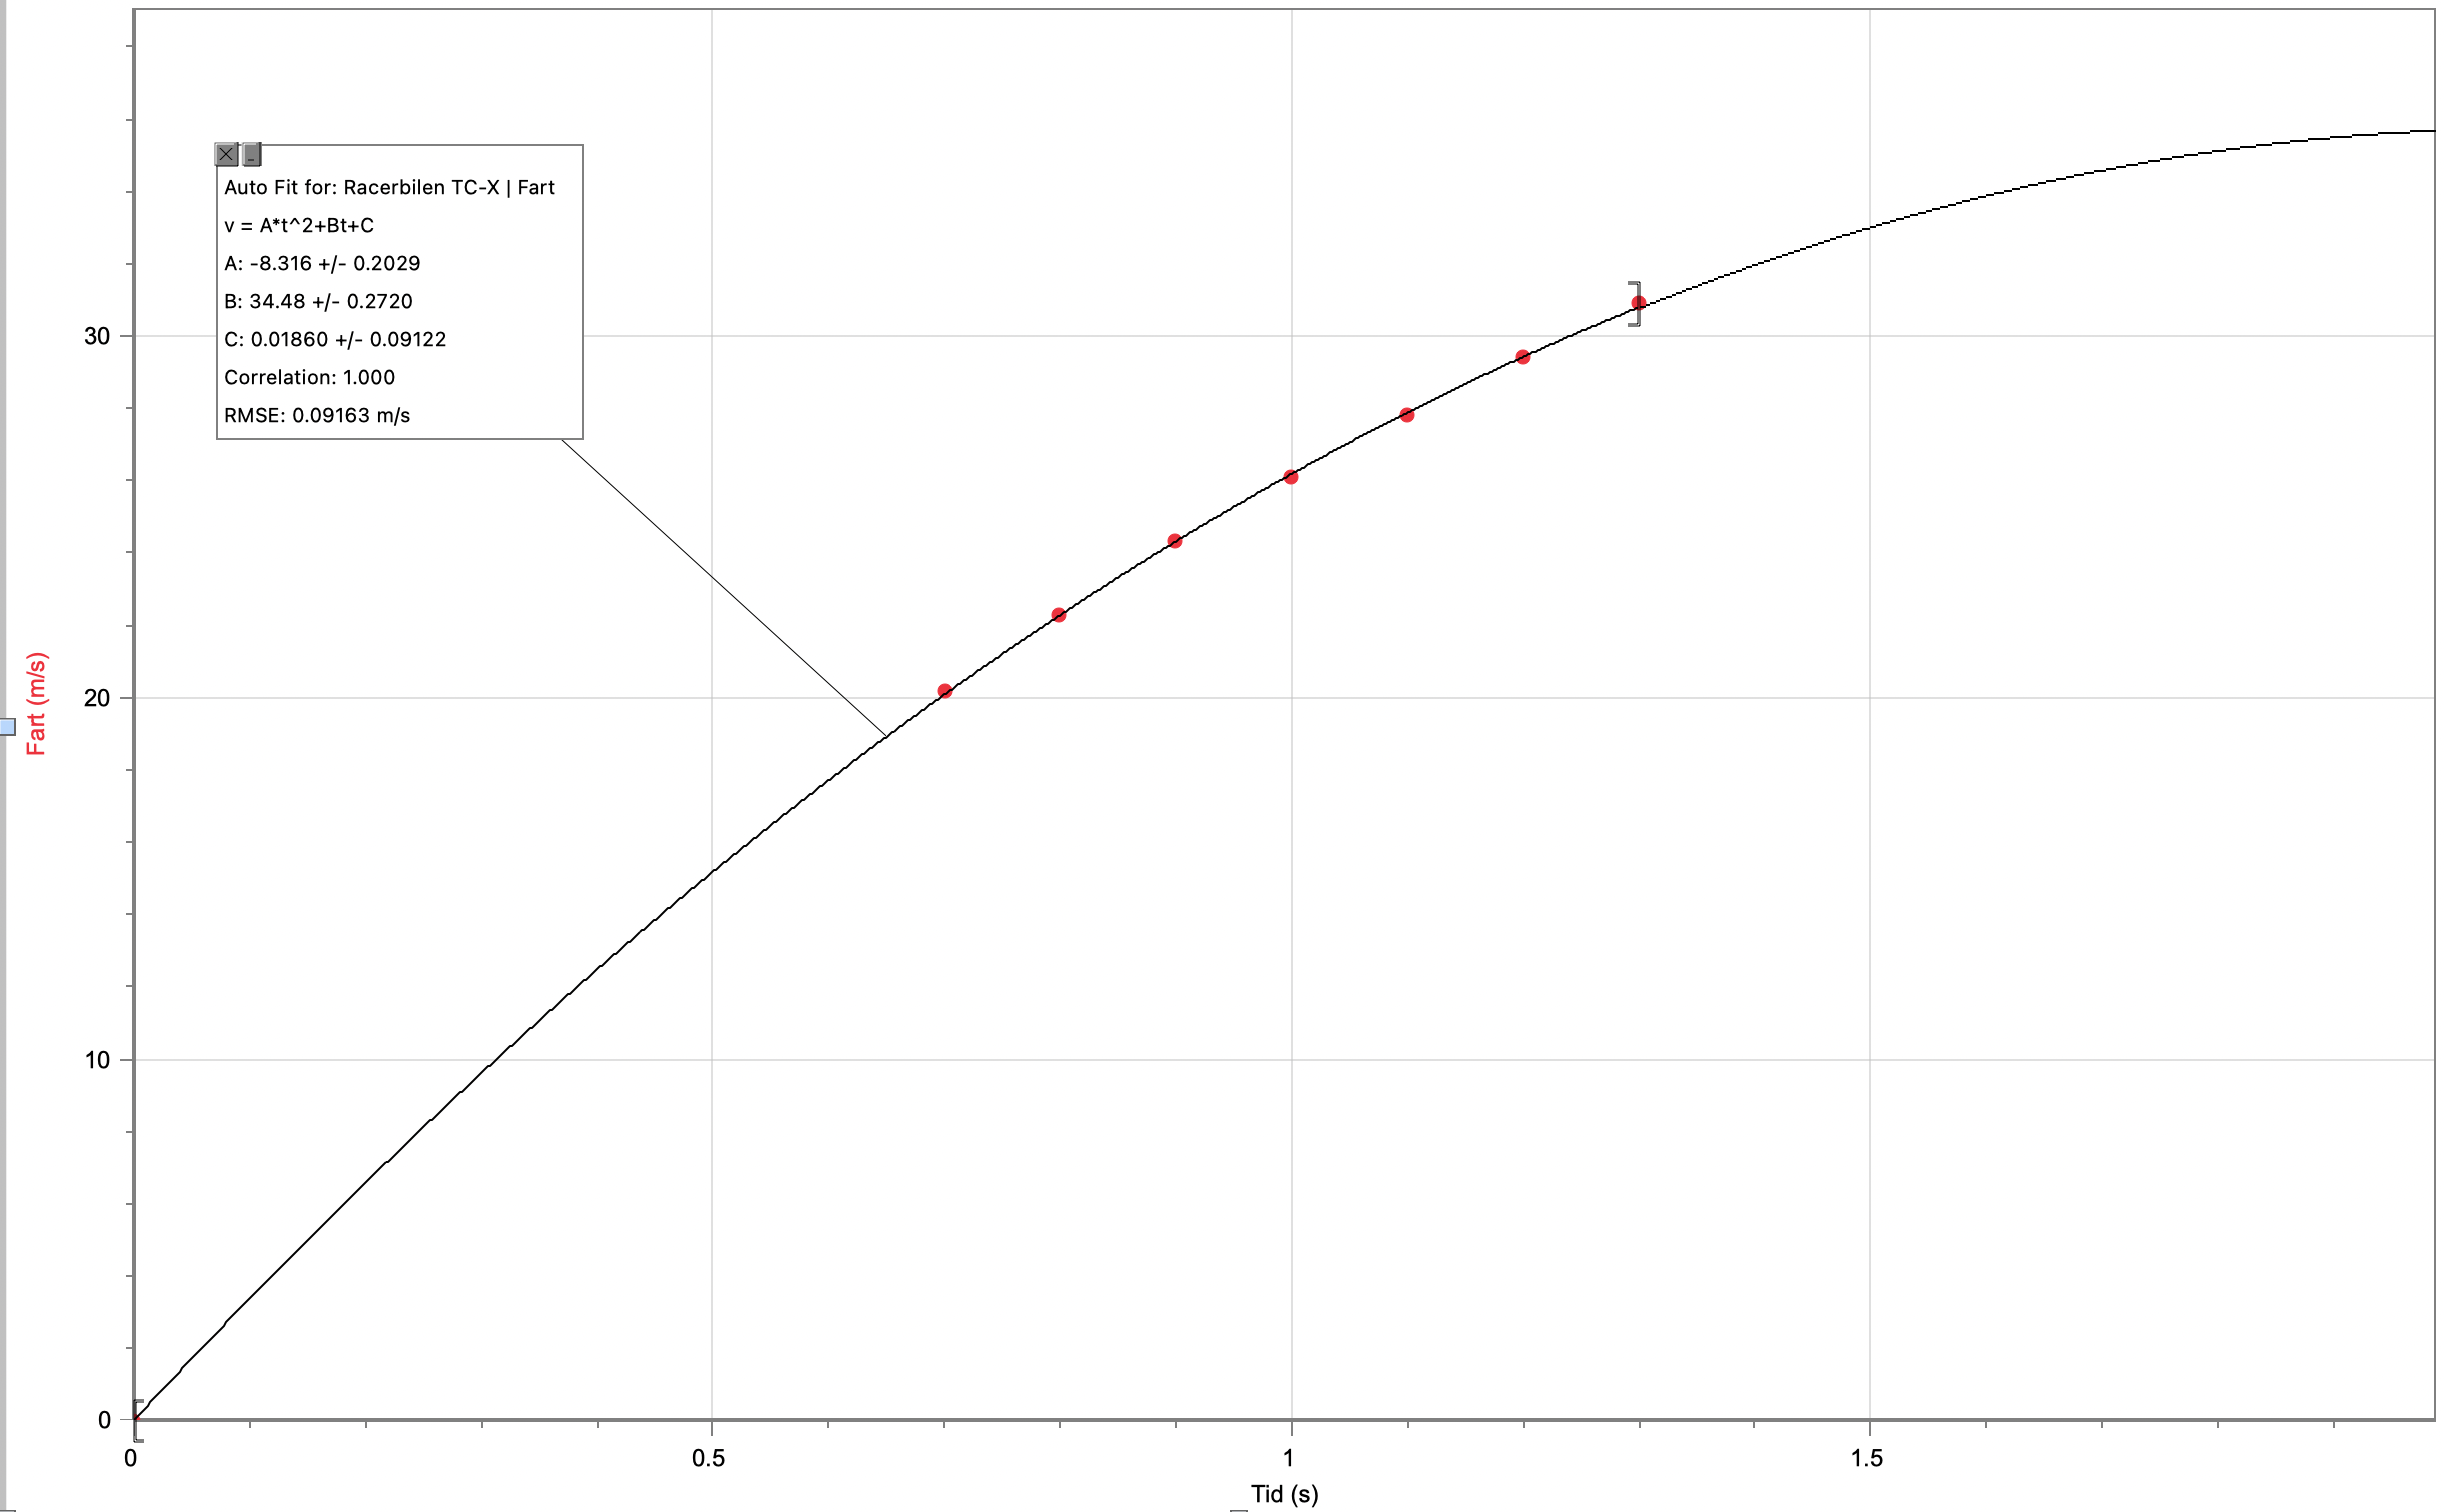
\includegraphics[scale=0.3]{H4_3.png}
\end{center}
  \caption{Fit med andengradspolynomium efter tilføjelse af punktet (0,0)}
\label{fig:3}
\end{figure}
\pagebreak

\begin{question}{}{}
  Fra tidspunktet $0,800\;\unit{s}$ efter start og til slutningen af rekordforsøget drives elbilen TC-X frem af en samlet kraft, sådan at dens stedfunktion følger modellen
\[
  s(t)=-0,6733\;\unit{m/s^3} \cdot t^3+10,95\;\unit{m/s^2} \cdot t^2+6,100\;\unit{m/s}\cdot t - 12,22\;\unit{m}
\] 
\begin{itemize}
  \item[i.] Check, om oplysningen om den tilbagelagte afstand i rekordforsøget faktisk passer med denne model.
\end{itemize}
\end{question}
\sol  \\ 
$t$ fra opgave 1 tages blot og sættes ind i funktionen, hvorefter der sammenlignes med afstanden.
\begin{equation*}
\begin{split}
s(4,897 \;\unit{s} )&= -0,6733\;\unit{m/s^3} \cdot (4,897 \;\unit{s})^3+10,95\;\unit{m/s^2} \cdot (4,897 \;\unit{s})^2+6,100\;\unit{m/s}\cdot 4,897 \;\unit{s}  - 12,22\;\unit{m}\\ 
&\approx 201,2 \;\unit{m} 
\end{split}
\end{equation*}
Dette var da netop afstanden, som TC-X tilbagelagde. Altså passer oplysningen om den tilbagelagte afstand i rekordforsøget med modellen.

\begin{question}{}{}
\begin{itemize}
  \item[j.] Bestem fartfunktionen $v(t)$ ved differentiation af ovenstående model for stedfunktionen $s(t)$.
\end{itemize}
Ved afslutningen af rekordforsøget, målte man bilens fart til $64,9 \;\unit{m/s} $
\begin{itemize}
\item[k.] Passer modellen for fartfunktionen i delopgave j. med den målte fart?
\end{itemize}
\end{question}
\sol \\ 
Fartfunktionen er den afledede funktion af $s(t)$.
\begin{equation*}
\begin{split}
  v(t)=\dv{t}\left(s(t)\right)&=3\cdot(-0,6733\;\unit{m/s^3}) \cdot t^2+ 2\cdot 10,95\;\unit{m/s^2} \cdot t+6,100\;\unit{m/s}\\ 
  &= -2,0199 \;\unit{m/s^3}  \cdot t^2 + 21,90 \;\unit{m/s^2} \cdot t + 6,100 \;\unit{m/s}  
\end{split}
\end{equation*}
For at tjekke om modellen passer med den målte data, sætter vi endnu engang blot tiden ind i funktionen, hvorefter vi sammenligner med bilens målte fart.
\begin{equation*}
\begin{split}
  v(4,897 \;\unit{m/s} ) &=-2,0199 \;\unit{m/s^3}  \cdot (4,897 \;\unit{m/s})^2 + 21,90 \;\unit{m/s^2} \cdot 4,897 \;\unit{m/s} + 6,100 \;\unit{m/s}\\ 
  &\approx 64,91 \;\unit{m/s}\\ 
  &\approx 64,9 \;\unit{m/s} 
\end{split}
\end{equation*}
Altså passer modellen for fartfunktionen med den målte fart.
\end{document}
